%%%%%%%%%%%%%%%%%%%%%%% file template.tex %%%%%%%%%%%%%%%%%%%%%%%%%
%
% This is a general template file for the LaTeX package SVJour3
% for Springer journals.          Springer Heidelberg 2010/09/16
%
% Copy it to a new file with a new name and use it as the basis
% for your article. Delete % signs as needed.
%
% This template includes a few options for different layouts and
% content for various journals. Please consult a previous issue of
% your journal as needed.
%
%%%%%%%%%%%%%%%%%%%%%%%%%%%%%%%%%%%%%%%%%%%%%%%%%%%%%%%%%%%%%%%%%%%
%
% First comes an example EPS file -- just ignore it and
% proceed on the \documentclass line
% your LaTeX will extract the file if required
\begin{filecontents*}{example.eps}
%!PS-Adobe-3.0 EPSF-3.0
%%BoundingBox: 19 19 221 221
%%CreationDate: Mon Sep 29 1997
%%Creator: programmed by hand (JK)
%%EndComments
gsave
newpath
  20 20 moveto
  20 220 lineto
  220 220 lineto
  220 20 lineto
closepath
2 setlinewidth
gsave
  .4 setgray fill
grestore
stroke
grestore
\end{filecontents*}
%
\RequirePackage{fix-cm}
%
%\documentclass{svjour3}                     % onecolumn (standard format)
%\documentclass[smallcondensed]{svjour3}     % onecolumn (ditto)
\documentclass[smallextended]{svjour3}       % onecolumn (second format)
%\documentclass[twocolumn]{svjour3}          % twocolumn
%
\smartqed  % flush right qed marks, e.g. at end of proof
%
\usepackage{amsmath}
\usepackage{graphicx} % Allows including images
\usepackage{algorithm}
\usepackage{algpseudocode}
\usepackage[round]{natbib}
\setcitestyle{aysep={ }} %Author-Year SEParator
%
% \usepackage{mathptmx}      % use Times fonts if available on your TeX system
%
% insert here the call for the packages your document requires
%\usepackage{latexsym}
% etc.
%
% please place your own definitions here and don't use \def but
% \newcommand{}{}
%
% Insert the name of "your journal" with
% \journalname{myjournal}
%
\begin{document}

\title{Learning Discrete-valued Bayesian Network from Mixed Data%\thanks{Grants or other notes
%about the article that should go on the front page should be
%placed here. General acknowledgments should be placed at the end of the article.}
}
%\subtitle{Do you have a subtitle?\\ If so, write it here}

%\titlerunning{Short form of title}        % if too long for running head

\author{First Author         \and
        Second Author %etc.
}

%\authorrunning{Short form of author list} % if too long for running head

\institute{F. Author \at
              first address \\
              Tel.: +123-45-678910\\
              Fax: +123-45-678910\\
              \email{fauthor@example.com}           %  \\
%             \emph{Present address:} of F. Author  %  if needed
           \and
           S. Author \at
              second address
}

\date{Received: date / Accepted: date}
% The correct dates will be entered by the editor


\maketitle

\begin{abstract}
Insert your abstract here. Include keywords, PACS and mathematical
subject classification numbers as needed.
\keywords{Discretization \and Bayesian Network \and More}
% \PACS{PACS code1 \and PACS code2 \and more}
% \subclass{MSC code1 \and MSC code2 \and more}
\end{abstract}

\section{Introduction}
\label{intro}
Bayesian networks \citep{Pearl_1988, PGM_2009}  are an increasingly popular methods for modeling uncertainty and causality in science and engineering. They provide an efficient factorization of the joint probability distribution over a set of random variables. Bayesian networks first emerge from artificial intelligence research and have been applied to a wide variety of problems, ranging from decision-making systems \citep{DMU_2015} to medical diagnoses. In most cases, we assume that all random variables in Bayesian networks are discrete, since many algorithms on Bayesian networks are unable to deal with continuous variables efficiently. However, this assumption is often too restrictive. For example, in the decision-making system of autonomous cars, it is inevitable to deal with continuous variables such as position and velocity. 

There are two solutions around this assumption. The first one is to model conditional probability density of each continuous variable by specific families of parametric distributions, then redesign algorithms on Bayesian networks based on these parameters. One successful example is the belief propagation in Gaussian graphical models \citep{Weiss_2011}. Nevertheless, for other shapes of particles \citep{Ihler_2009} or non-linear functions, algorithms are computationally expensive and do not perform well.

The second solution is to discretize continuous variables. Discretization that learns from data has developed well and discussed \citep{Dougherty_1995} in the fields of machine learning and statistics for many year. Most of these discretization methods are designed for classification problems. They search the best discretization of a continuous attribute by considering its interation with the class variable of interest. However, these discretization methods do not apply to continuous variables in Bayesian network. In Bayesian network, interations and dependencies between variables are determined by graph structure. Therefore, if a discretization method only uses the interation between a continuous variable and its class variable of interest, instead of considering the graph structure, then it is not an appropriate discretization method for Bayesian networks. There are some reseach on discretizating continuous variables in naive Bayesian network and tree augmented network \citep{Fried_naive}. Nevertheless, only few discretization methods on general Bayesian netowrk have been proposed \citep{Friedman_1996, Kozlov_1997, Monti_1998}.

The discretization technique proposed by N. Friedman and M. Goldszmidt \citet{Friedman_1996} is the most successful and practical one among these methods. It is based on minimum description length principle (MDL): optimal discretization policy minimizes the description length of Bayesian network and data information. If there is only one continuous variable in Bayesian network and other variables are discrete, MDL discretization method takes running time $O(N^3 + n_c {v_{max}}^{(n_c^p)_{max}} \cdot N^2 + {v_{max}}^{n_p} \cdot N^2)$, where $N$ is the number of data instances for learning the discretization, $n_p$ and $n_c$ are the numbers of parent and children variables for the continuous variable, $v_{max}$ is the largest cardinality number over all variables in Markov blanket, and  ${(n_c^p)_{max}}$ is the largest number of parent variables of the continuous variable's children.

In this paper, we propose a new discretization method for continuous variables in Bayesian network by learning from mixed data. This method is a generalized version of  \citet{Boulle_2006} and \citet{Lustgarten_2011}, which are both discretization methods of a continuous attribute with one class variable. We begin our method with the situation that only one variable in a given Bayesian network is continuous and other variable are discrete. Under this situation, we look for the most possible discretization policy $M$ given the data on other discrete variables. That is to say, the desired policy is $\textrm{arg}_M P(M|D)$. With Bayes rule, $P(M|D) = P(M) \cdot P(D|M) / P(D) \propto P(M)\cdot P(D|M)$. Usually, $P(D|M)$ increases as number of discretized intervals increases, since more intervals can provide more accuracy. Therefore, we design probability priors of $P(M)$ to decrease as number of intervals rises. As a result, we obtain a nature trade-off to determine the number of intervals after discretization. Besides, the $P(D|M)$ can be factorized according to Bayesian network structure. On the other hand, with the proposed priors, we are able to restrict the number of discretized intervals not exceeding the largest cardinality number of variable in Markov blanket too much. This is important, since for most algorithms on Bayesian network, their running times exponentially depend on the cardinality of variables. Another advantage of our algorithm is running time. If there is only one continuous variable, the running time is $O(n_c  {v_{max}} \cdot N^2 + {v_{max}}^{n_p} \cdot N^2)$, which beats the running time of MDL principle discretization \citep{Friedman_1996}. With an effective approximation proposed in this paper, we can further reduce running time to $O({v_{max}}(n_p+n_c)N^2)$.

For a Bayesian network with multiple continuous variables, we apply the discretization method discussed above iteratively. In the beginning, we discretize each continuous variable by equal-width method. Number of intervals for equal-width discretization is equal to largest cardinality of discrete variables. Then we iterate the one-variable discretization on each continuous variable by the following order: from the variable with highest topological order (leaves) to the variable with lowest topological order (root). Everytime when we finish a discretization procedure on one variable, we store the discretization result and this discretization result will be used for later discretization on another variable. Experiments on real data show that with same iteration order, our discretization provides better discretization result than MDL principle method in terms of likelihood. The latter is easily catched by local minima and thus produce non-necessarily low number of intervals after discretization.

Finally, we can combine the new discretization method with K2 structure learning alorithm \citep{K2}. We first prediscretize all continuous variables before K2 learning, since K2 algorithm requires all variables are discrete. Everytime when an edge is added by K2 algorithm procedure, we rediscretize the relevant variables in Bayesian network and store the result for next K2 algorithm iteration. By this principle, we are able to learn a discrete-valued Bayesian network from mixed data.

The rest of the paper is organized as follows: we prepare the preliminaries and notations of Bayesian network in Section 2. Related work, including MDL principle discretization \citep{Friedman_1996} and MODL discretization by \citet{Boulle_2006}, are summarized in Section 3. In Section 4, we introduce the new discretization method, including formulation of objective function and algorithms. One continuous variable case and multiple continuous variable case are also included in this section. Finally, in Section 5, we apply the new discretization method to real-world data and show the result.
%
%\section{Related Work}
%\label{relat_work}
%
%\section{Notation and Preliminaries}
%\label{notat_pre}
%\subsection{Bayesian Network}
%\label{BN}
%A Bayesian network $B$ is defined by a pair $(G,\Theta)$, where $G = (X,E)$ is a directed acyclic graph whose nodes correspond to a set of random variable $X = \{  X_1, X_2, \cdots, X_n \}$, and whose edges $E$ represents probabilistic dependencies among nodes. The graph structure $G$ encodes the Markov property: each node $X_i$ is independent of its non-descendants given its parents in $G$. The second component of $B$, namely $\Theta$, contains a set of parameter that qualifies the network. Elements of $\Theta$ take the form $\theta_{x_i|\Pi_{x_i}} = P(x_i|\Pi_{x_i})$ for each possible value $x_i$ of $X_i$, and $\Pi_{x_i}$ of $\Pi_{X_i}$ (the set of parents of $X_i$ in $G$). Due to Markov property, we can represent the multivariate joint distribution over $X$ as
%\begin{equation*}
%P_B (X_1 , \cdots, X_n) = \prod_{i=1}^{n} P_B (X_i | \Pi_{X_i}) = \prod_{i=1}^{n} \theta_{x_i|\Pi_{x_i}}
%\end{equation*}\\
%For a Bayesian network, we can generate its data instances by forward sampling, i.e., sampling variables one by one in a topological order. A topological order is obtained by breadth-first search. Given a instance of $X_i$'s parent set $\Pi_{X_i}$, value of $X_i$ can be sampled according to conditional probability relation $P(X_i | \Pi_{X_i})$. Furthermore, this parent-child sampling order can be reversed if we know the marginal probability of child variable $P(X_i)$. By Bayes rule,
%\begin{equation*}
%P(X_i | \Pi_{X_i}) \cdot \prod_{j = 1}^{ Pa( X_i)} P( \{ \Pi_{X_i} \}_j) = P(X_i) \cdot P(\Pi_{X_i} | X_i),
%\end{equation*}
%where $Pa( X_i)$ is the number of parents of $X_i$, we can first sample $X_i$ by $P(X_i)$, then sample the parent varaibles simultaneously by $P(\Pi_{X_i} | X_i)$. That is to say, $X_i$ becomes the starting point for sampling. $X_i$'s descendants are sampled in the same way as forward sampling. $X_i$'s ancestors are sampled in a reverse order.
%\subsection{K2 Structure Learning}
%\label{K2}
%
%\section{Section title}
%\label{sec:1}
%\subsection{Subsection title}
%\label{sec:2}
%as required. Don't forget to give each section
%and subsection a unique label (see Sect.~\ref{sec:1}).
%\paragraph{Paragraph headings} Use paragraph headings as needed.
%\begin{equation}
%a^2+b^2=c^2
%\end{equation}

% For one-column wide figures use
\begin{figure}
% Use the relevant command to insert your figure file.
% For example, with the graphicx package use
  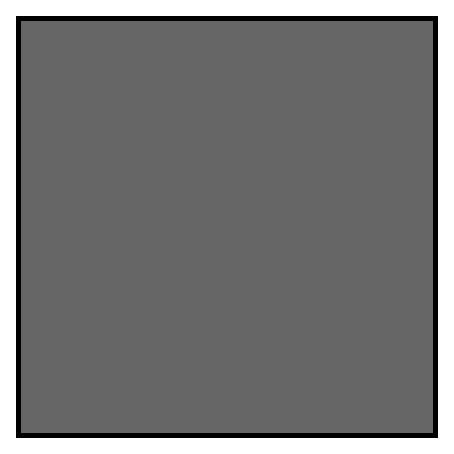
\includegraphics{example.eps}
% figure caption is below the figure
\caption{Please write your figure caption here}
\label{fig:1}       % Give a unique label
\end{figure}
%
% For two-column wide figures use
\begin{figure*}
% Use the relevant command to insert your figure file.
% For example, with the graphicx package use
  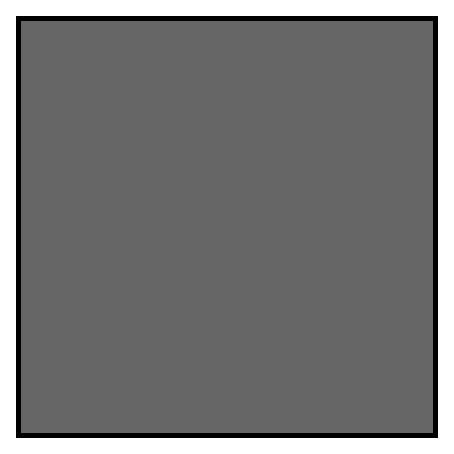
\includegraphics[width=0.75\textwidth]{example.eps}
% figure caption is below the figure
\caption{Please write your figure caption here}
\label{fig:2}       % Give a unique label
\end{figure*}
%
% For tables use
\begin{table}
% table caption is above the table
\caption{Please write your table caption here}
\label{tab:1}       % Give a unique label
% For LaTeX tables use
\begin{tabular}{lll}
\hline\noalign{\smallskip}
first & second & third  \\
\noalign{\smallskip}\hline\noalign{\smallskip}
number & number & number \\
number & number & number \\
\noalign{\smallskip}\hline
\end{tabular}
\end{table}


%\begin{acknowledgements}
%If you'd like to thank anyone, place your comments here
%and remove the percent signs.
%\end{acknowledgements}

% BibTeX users please use one of
%\bibliographystyle{spbasic}      % basic style, author-year citations
%\bibliographystyle{spmpsci}      % mathematics and physical sciences
%\bibliographystyle{spphys}       % APS-like style for physics
%\bibliography{}   % name your BibTeX data base

% Non-BibTeX users please use
%\begin{thebibliography}{}
\bibliographystyle{plainnat}
\bibliography{my_bib}

\end{document}
% end of file template.tex

